\chapter{Methods}\label{chapter:methods}

This chapter describes implementation of the mobile Augmented Reality (AR) pipeline of avatars rendering, and experiments on increasing the DNN's \cite{dnn:stylepeople21} images quality for AR scenario. Section \ref{methods:dev-setup} lists target hardware and software, including the used libraries, tools, and configuration of the baseline model. Section \ref{methods:app} describes the mobile pipeline and algorithmic tricks used to achieve real-time performance. Section \ref{methods:zooms} presents motivation and implementation details for experiments with the DNN's training procedure.

\section{Experimental setup}\label{methods:dev-setup}

The baseline DNN \cite{dnn:stylepeople21} model can be trained on a monocular video sequence of frames with a single person shown from multiple sides. There are several pre-made training video sequences with different people at our disposal. They were captured for approximately 1 minute on a stationary monocular smartphone camera, in resolution $1920 \times 1080$ pixels. Only each 8th frame from the video was retained to get a representative set of distinct body poses. Then, for each frame a segmentation mask was predicted using an external pretrained segmentation model Graphonomy \cite{dnn:graphonomy19}, to replace color of background objects with 0 values. Next, SMPL-X \cite{dnn:smplx19} body model was fit to all the frames, i.e. predicting pose vector $\theta$, facial expression vector $\psi$, and body shape vector $\beta$. The latter is purposely predicted to be the same across all the frames, in order to bias the DNN to synthesize images for this body shape only, which will be exploited in real-time inference on mobile in Section \ref{methods:app}. Using body model fits, a posed body mesh for each frame can be obtained as was described in Section \ref{lit:nrender}. 

Sometimes, 3D model fits may be misaligned with complicated ground truth 2D frames, e.g. due to complex twists and bending of joints, occluded body parts. To reduce the effect of training the DNN on outlying unstable inputs, many of the falsely fit ground truth images were manually filtered out from the training set. It was observed, that the quality of body model fits is critical for the avatars final quality. Hence, for the scope of this thesis, we decided to take a single training sequence, that has the best body model fits we could obtain. The training pipeline adjustments discussed in Section \ref{methods:zooms} will be primarily applied to this training sequence. This also allows the fair quantitative and qualitative comparison. For simplicity, when we further mention \textit{the training sequence}, we mean this single training sequence. A few promising experiments will be repeated with a few other sequences to verify stability of results (for example, see Figure \ref{fig:exp:instancenorm-other-seq}). 

After filtering out the bad frames, the training sequence contains 410 samples. Out of them we holdout 13 frames as a validation set. It includes 11 consecutive frames from a frontal view, in poses that do not resemble any other training data; and also 2 frames with side and back view. As for a test set, we made a sequence of continuous difficult poses and camera angles. It includes an animation with extensive hands gesturing, a view on the avatar from top, bottom, far away, and close-up to the face. The test sequence is completely unrelated to the training data and was designed by us to verify that the DNN is capable of rendering frames that may be encountered by a user in an AR session. The possible visual artifacts may include flickering between two similar frames, clothes shaking, color shifts, blurriness, etc. See Appendix Section \ref{appb:exps}, featuring a few training and test images that we use. Lacking an absolute metric of visual quality, in this research we mainly rely on manual inspection and comparison of the test video sequences. 

In the next paragraphs we will elaborate more on the specific configuration of the baseline DNN architecture, that was first mentioned in Section \ref{lit:nrender}. By default, we stick to $512\times512$ pixels resolution of synthesized images. Both the ResNet18 encoder and decoder of the neural renderer consist of 5 levels of 2-layer CNNs with stride 2 and kernel sizes either $3\times3$ or $5\times5$. The U-Net yields a tensor with 64 channels and the original spatial resolution. Two independent CNNs with 2 layers each (also called heads) then map it into a 3-channel RGB image, and a 1-channel segmentation mask, that are concatenated into the final RGBA avatar image.

%$C \times 512 \times 512$ ($C$ is number of input channels and $512 \times 512$ is spatial resolution) is enlarged to $64$ channels, and processed by 5 sequential levels, each consisting of 2 convolutional layers. Through the levels, the size of activations follows the sequence: $64 \times 256 \times 256 \rightarrow 128 \times 128 \times128 \rightarrow 256\times64\times64 \rightarrow 512\times32\times32$. The resulting activation is then passed through the decoder part, where it gets upsampled to twice as bigger spatial resolution, then it is concatenated with the second to last encoder level's activations. The decoder level ends with a convolutional layer. The same procedure is repeated for the remaining decoder levels, concatenating with features of the corresponding encoder levels. Finally, on tensor size $64\times512\times$, the channels depth is shrunk to 16, and .

The neural texture is a tensor of 16 channels and resolution $512\times512$ by default (although may be arbitrary). For the SMPL-X body model mesh, there is a known mapping from 3D mesh vertices to the same 2D texture image coordinates (as on Figure \ref{intro:fig:mesh-texture}), regardless of body shape (tall, short, slim or obese). In addition to the original resolution, extra texture scales of size $16\times 2^k \times 2^k, \forall k \in \{3,..,8\}$ are created and jointly optimized. This set of scales is referred to as a multi-scale neural texture. Before rasterizing the body mesh, all the scales are upsampled to $512$ resolution and averaged into a single texture. The multi-scale texture allows to share information among adjacent vertices and proven to reduce flickering of the output avatar images. Also, the baseline neural texture uses a special initialization. It is computed as spectral coordinates of vertices on the graph, that is made out of the body mesh. In short, the graph's Laplacian matrix is calculated, and Eigenvectors of it are called spectral coordinates \cite{aux:spectral10}. A few first dimensions of these vectors are used to initialize the neural texture. The purpose of such initialization is in separation between different parts of the body (see Figure \ref{fig:spectral_ntex}), e.g. there are channels that assign opposite values to left/right limbs, or lower/upper body, or adjacent fingers and so on. Such initialization helps to guide the neural renderer to uniquely distinguish the body parts, improving convergence speed.

During training, the synthesized image and its segmentation mask are supervised with a weighted sum of training losses. By default Dice, L1, LPIPS (VGG \cite{dnn:vgg14} based), Adversarial and Feature Matching losses are used, with weights 25, 25, 20, 1, 1 respectively. The adversarial loss is a Binary Cross Entropy (BCE) loss of predictions made by an ensemble of $N=3$ discriminator networks. Each discriminator is a CNN that gradually decreases the spatial resolution and increases the number of channels, until finally a Sigmoid function returns a probability in range $[0;1]$ of the image being real. The discriminators are supervised to improve their accuracy on both synthesized and real images, while the neural renderer is supervised to decrease discriminators' accuracy for the synthesized ones. See Formula \ref{methods:eq:bce} for BCE, when computing it for a real image $x$, then $y$ is set 1 for discriminators; if $x$ is a generated image, then $y$ is 0 for discriminators, but 1 for the neural renderer.
\begin{equation}
	BCE = - \dfrac{1}{N} \sum_{i=0}^N y \cdot \log_{2}(D_i(x)) + (1-y) \cdot \log_{2}(1 - D_i(x)) 
	\label{methods:eq:bce}
\end{equation}

Adam \cite{dnn:adam14} optimizer is utilized for training of the neural renderer, neural texture and discriminators. They are optimized with learning rate (LR) of $10^{-3}$, $10^{-3}$ and $10^{-5}$ respectively. By default, the Adam's first and second momentum values are 0.9 and 0.999 respectively, without weight decay (also known as L2 penalty on norm of the optimized parameters).

In the baseline training process, a batch of random training samples is selected. Using body model's mesh, a bounding box is found that tightly encloses the person's extents on the ground truth image. The image is cropped by this bounding box using bilinear interpolation to get a $512 \times 512$ image with the person's body in the image center. With the same resolution and alignment, the body mesh is rasterized. Then, both the ground truth and rasterization are processed with image-space augmentations (see Figure \ref{fig:image-space-aug-kornia}), that perform random affine rotation, scale and translation of the image to improve generalization of the neural renderer to different camera views on the same avatar. Then the neural renderer is infered with input rasterization, and loss is computed between real and synthesized images. The gradient is computed and applied to all the learned parameters (the neural texture, neural renderer and discriminators) on every single batch. We train the pipeline on desktop hardware -- one GPU NVIDIA Tesla P40. It takes about 16 hours to complete a single experiment of 500 epochs on about 500 frames of ground truth images, with batch size 8 and resolution $512\times512$ pixels. All training computations are carried out in full-float FP32 numbers format. As validation metrics, we compute LPIPS (AlexNet \cite{dnn:alexnet12} based), SSIM, MS-SSIM, and PSNR, as well as tracking values of L1, Adversarial and Dice losses on the validation set.

The experimentation on deep neural networks is carried out in Python programming language and PyTorch framework for the DNNs training. We use many Python libraries for data processing and visualization: NumPy, Matplotlib, OpenCV, Pillow, Open3D. In order to optimize parameters of the neural texture, it needs to be rasterized with the body mesh using differentiable rendering algorithm, we use Nvdiffrast library for that \cite{aux:nvdiffrast20}. The image-space augmentations need to be differentiable for the same reason, for which we utilize Kornia library \cite{aux:kornia20}.

The primary mobile hardware that we target with our mobile application is SoC Qualcomm Snapdragon 888, which is one of the latest high-end platforms that features a fast and power efficient DSP computing unit for AI, and high throughput for processing mobile camera data in real-time. Although the preceding versions of the platform also contain the DSP, they are too slow to infer the baseline DNN in real-time. Qualcomm Snapdragon 835 is the oldest platform that we succeeded to launch the mobile application on, although with unacceptable performance.

We develop the mobile application in Java and Kotlin programming languages. The development environment consist of the Java Software Development Kit (SDK) and Android SDK. We perform installation of the compiled code on a mobile device via Android Debug Bridge (ADB) software utility. In order to launch the PyTorch DNN on mobile, first of all we use Snapdragon Neural Processing Engine SDK (SNPE, \cite{aux:snpe}). It includes Android runtime libraries, as well as desktop software tools for conversion of DNN architectures into binary files, that can be loaded onto mobile devices and executed. Among the tools there is a utility for post-training quantization of a neural architecture. We supply it with 5-10 input frames from the test sequence. The neural renderer network is inferred with those frames, and the range of quantization is computed for each intermediate tensor. Then all the weights are quantized as was described in Section \ref{lit:dnn-speedup}. The direct conversion of PyTorch DNN models into SNPE format is not supported, however there is an Open Neural Network Exchange format (ONNX, \cite{aux:onnx}), which supports conversion from PyTorch to ONNX (provided by PyTorch), and from ONNX to SNPE (provided by SNPE SDK). The final file with the quantized DNN is passed along with the quantization constants to the mobile application to accordingly generate quantized input frames.

On the mobile application's side, we use SNPE Android Runtime library to load the model's file and to specify performance profiles. Those control how much of computing power should be devoted by the device. We use "Sustained High Performance" profile, since we intend to continuously infer the DNN over a long period of time with low latency. On the other hand, there is the absolute highest performance profile, that would lead to the best performance over a short period of time, that would drastically decrease upon reaching the overheating limit. Prior to inference, SNPE should be given with pointers to memory locations, where to read the input data, and where to write the output data. We accordingly preallocate buffers on CPU and GPU, and use them for the whole run of the mobile application to minimize costs of memory allocation on each frame.

For the DNN inference, we need to generate an input frame (see Figure \ref{lit:fig:stylepeople}), that would show the body mesh oriented as an object of Augmented Reality. Hence, the orientation should correspond to the mobile device's camera. This requires continuous tracking of camera position in the real world, as well as positions of the surrounding environment. We use ARCore SDK \cite{aux:arcore22} that provides it with little programming required. It uses inertial measurement units, camera images and depth sensor of the device to keep track of distinct points in the camera view. This allows to estimate proximity of the real world objects, and to reconstruct vertical and horizontal flat surfaces, such as floors, desks, walls. The location and bounds of these surfaces can be queried from the ARCore. It also allows to place and track anchor points on the detected surfaces. The tracking information can be retrieved from ARCore in a form of transformation matrices of the anchors and camera (extrinsics, as in Formula \ref{lit:eq:extrinsic}). The projection matrix of the camera (intrinsics, as in Formula \ref{lit:eq:intrinsic}) can also be retrieved, allowing to render images that span the whole screen of the device. 

The generation of input frames is in essence a classic rasterization of a triangular mesh onto an image using a 2D texture. This process can be delegated to the high-performance graphics library, which is called Open Graphics Library (OpenGL, \cite{aux:opengl22}). It provides low-level control of a GPU device, to layout and are pre-process the data of meshes and textures. Then, using GPU programs written in OpenGL Shading Language (GLSL, \cite{aux:glsl21}), also referred to as shader programs, we can make linear algebra computations on individual vertices of the mesh (vertex shader), or individual pixels on the rendered image (fragment shader). Since all those primitives can be processed independently, this computation is automatically parallelized on GPU by OpenGL, thus achieving very high performance of rasterization. We also use it to render camera frames on the screen. On top of them we render the avatar images, resulted from the DNN's inference (see Figure \ref{fig:mobile_example}).

The application is compiled with all performance optimizations enabled. The frame time of the mobile AR experience is measured directly in the application. We report timings of processing steps of the current frame via logging, namely: time of SMPL-X body mesh inference from a pose vector, time of rendering the DNN's input frame on GPU, time of delay between obtaining this data and receiving it on the DNN's side, time of DNN's inference, time of rendering the inferred outputs on the screen. However we notice, that by far the highest processing time is taken by the DNN inference step. To measure its timings more accurately, we created a separate mode for the application, which we call "benchmarking". In this mode, the only thing that is being calculated is continuous inference of the DNN for a few minutes with a constant random tensor of data. Thus, the computing device will be maximally utilized with the DNN inference only. We consider it an upper bound of the power consumption and heat generation. The benchmarking reports increase in temperature and average timing of DNN inference. We additionally use Qualcomm Snapdragon Profiler software. It allows to capture hardware metrics of a running mobile application. From that, we visualize occupation of computing devices over time, and reason about potential bottlenecks.

\section{Mobile application development}
\label{methods:app}

The Android mobile application was developed from scratch specifically for this Master thesis. A considerable amount of technical work was spent on implementing general functionality of the application. This includes:
\begin{itemize}
	\item system events handling, such as opening, closing, resuming from the operating system;
	\item requesting of system permissions on camera and hard drive storage;
	\item adding binary files into an installation package, including runtime libraries, files of quantized DNN models, neural textures, configuration files, assets for inference of SMPL-X, etc;
	\item setup of logging;
	\item reacting to user interaction, such as finger taps, swipes, pinch movements;
	\item populating user interface with options that allow selecting a particular DNN for inference, selecting options of DNN input generation, predefined animations, features of rasterization, etc. 
\end{itemize}

We publish only a part of the code base that is the most relevant to synthesis of avatar images on mobile, that is described in the following paragraphs (See Appendix \ref{appendix-code}).

We initialize OpenGL library, by creating a \verb|Surface| object from the Android SDK, that spans the whole screen of the device, and specifying it as a context of OpenGL to render to. This creates a separate execution thread on CPU, the commands of OpenGL (and thus GPU processing) be executed only from here. We configure the context to use 8-bit for colors channels of the screen and 32 bits for values in the Z-buffer. In OpenGL all the data is allocated on GPU as contiguous arrays, and the library has to be programmed how to interpret these arrays. The triangular meshes can be defined by a flat array of vertex attributes, where consecutive elements contain attributes of a single vertex. The most basic scenario is to pass an array of $\langle x, y, z, u, v\rangle$ with $xyz$ being a 3D vertex position in a local coordinate space of the modeled object, and $uv$ being texture coordinates of the vertex. Also, a connectivity array has to be provided in a form of indices. For example, an array of indices $\langle1, 2, 3, 2, 3, 4\rangle$ can be interpreted as a triangular mesh, with 1 triangle made of vertices in the attributes array, with indices 1, 2 and 3; and another triangle of vertices 2, 3 and 4. We use back-face culling throughout the rendering, meaning that OpenGL will not render triangles facing away from the camera, slightly improving performance by culling some triangles out of processing. To define which triangles are facing away, we specify to interpret vertex indices as clockwise triangles, meaning that a triangle of indices $\langle1, 2, 3\rangle$ will face towards the camera if and only if the vertices 1, 2 and 3 appear in a clockwise order after projecting on the screen. Overall, we use three separate triangular meshes, one for SMPL-X human body mesh (described further), and two "meshes" which are essentially rectangles. The first one will be rasterized, spanning the whole screen, and taking color values from a texture that contains a current camera frame. The other one is similarly rasterized, but at a location of the avatar, taking values from a texture loaded with output of the inferred DNN (See a debugging illustration from the mobile application on Figure \ref{fig:far_dynamic_crop_debug}).

OpenGL doesn't support generation or storage of images with more than 4 channels (Red-Green-Blue-Alpha only). To load the neural texture of $C$ channels on GPU first of all if it is a multi-scale texture, we average all the scales into a single $C \times 512 \times 512$ texture scale. Then we split it by 4 channels and load these parts as separate of arrays on GPU. We use FP16 format for storage, to a reduce memory footprint of the texture and hoping to get better utilization of texture memory caches inside GPU. OpenGL allows to apply an additional filtering algorithm on textures, to generate multiple scales of the texture, which are called MIP-maps (see Figure \ref{fig:mipmap}). Those can be used to render triangles that span very little area on the screen. The filtering prevents appearing of blurriness and aliasing artifacts resulted from bilinear sampling. Furthermore, anisotropic filtering can be applied to also generate stratched variants of scales to also solve artifacts of rendering triangles facing at steep angles to the camera (see Figures \ref{fig:anisotropic} and \ref{fig:anisotropic_result}). Both methods require extra texture memory: about x2 for MIP mapping, and up to x16 for anisotropic filtering, and slightly more processing time. However, given the small resolution of our textures and relatively low triangle count in the body model, the performance difference is negligible. We would like to clarify the confusing terminology -- a multi-scale texture exists only in the DNN pipeline in Python, and its scales are upsampled and averaged before rasterization; on the other hand in the mobile application MIP maps always remain at lower resolutions and a specific scale is automatically selected by a GPU driver to render a certain triangle.

Next we initialize a tracking session of ARCore library. It starts intercepting and processing the camera frames on GPU, allowing to refer to the camera data as an OpenGL texture. By default ARCore receives a new camera frame and awaits for the next. The application is then capped to latency of the device camera -- 30 frames-per-second (FPS) for our devices. We configure ARCore to never wait and process the current camera frame, regardless if it was already processed. This allowed us to cap the application to the Android's internal cap of 60 FPS.

As was mentioned in Section \ref{methods:dev-setup}, we initialize SNPE DNN models with "Sustained High Performance" profile, and the computing unit specified from the user interfaces (supporting either GPU or DSP). GPU offers better support of neural layers used in DNN models, since it can perform computations in FP32 or FP16 format, analogously to a desktop GPU. But running a DNN on it would also mean that input rasterization and DNN inference would have to be done sequentially, possibly bottlenecking the performance. On the other hand, DSP offers much higher performance than of GPU, and inference can take place independently and in parallel with our input generation on GPU. However the usability of DSP is very limited, e.g. much fewer neural layers support quantized computations and also loading the DNN models requires long initialization, up to several minutes. Besides, Qualcomm Snapdragon's DSP contains a hardware security policy, that allows to run on DSP of consumer devices the code, that was certified by the hardware vendor. We ignore this issue for our project, by having test engineering samples of smartphones that suppress this security check. If SNPE fails to load a model on DSP, it may fallback to using GPU, or even CPU execution, obviously being extremely slow for inference.

Computing SMPLX rest pose mesh, selecting top joint weights

After initialization, the application enters an infinite loop of computing and rendering the AR experience. Each frame start from extracting tracking information from the ARCore session, namely camera intrinsic and extrinsic matrices, as well as transformation matrices of tracked anchors, surfaces, and their bounds. Unlike the classic 

...

Finally, we draw all the AR content on the screen - the camera frame, the tracked surfaces planes, and the synthesized avatar image at the frame coordinates calculated from the frustum crop.


\begin{figure}[ht]
	\centering
	%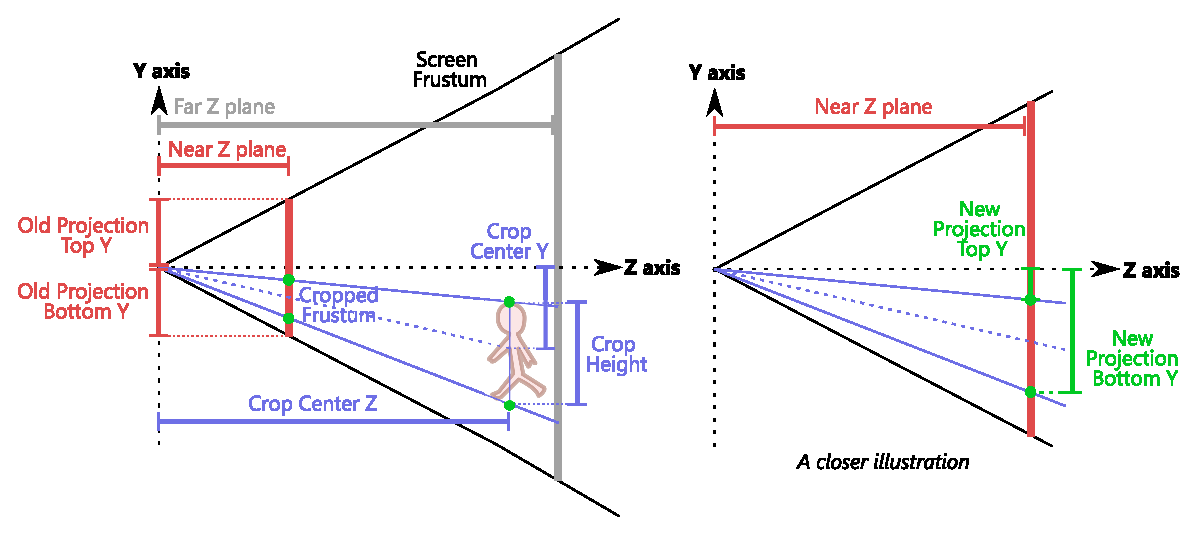
\includegraphics[width=\textwidth]{\imgfp/dynamic_crop/dynamic_crop}
	%\setkeys{Gin}{draft}
	\centering{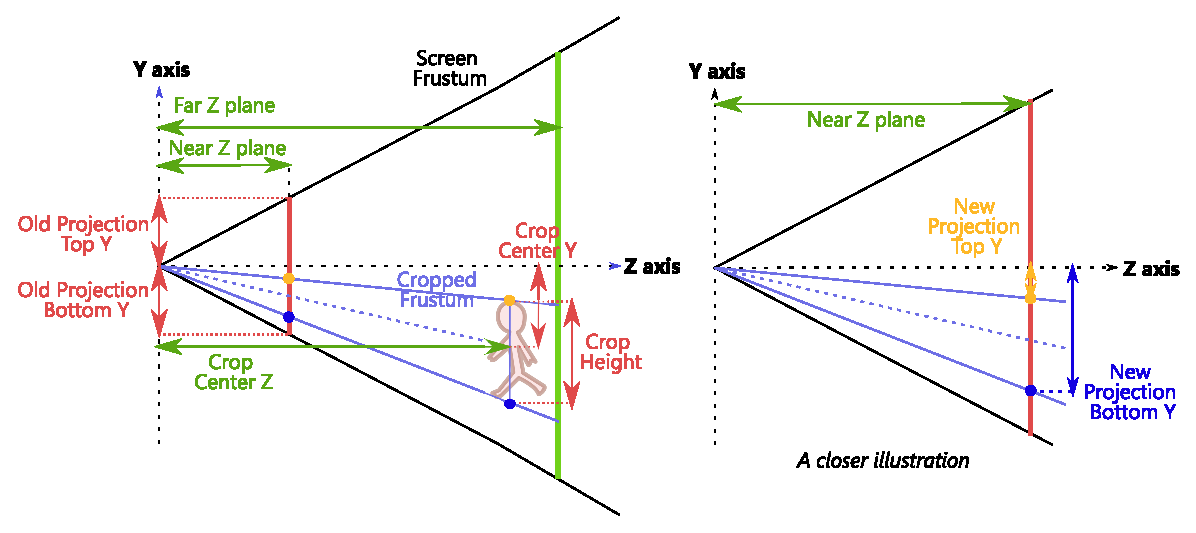
\includegraphics[width=\textwidth]{\imgfp/dynamic_crop/dynamic_crop_vect}}
	%\setkeys{Gin}{draft=false}
	%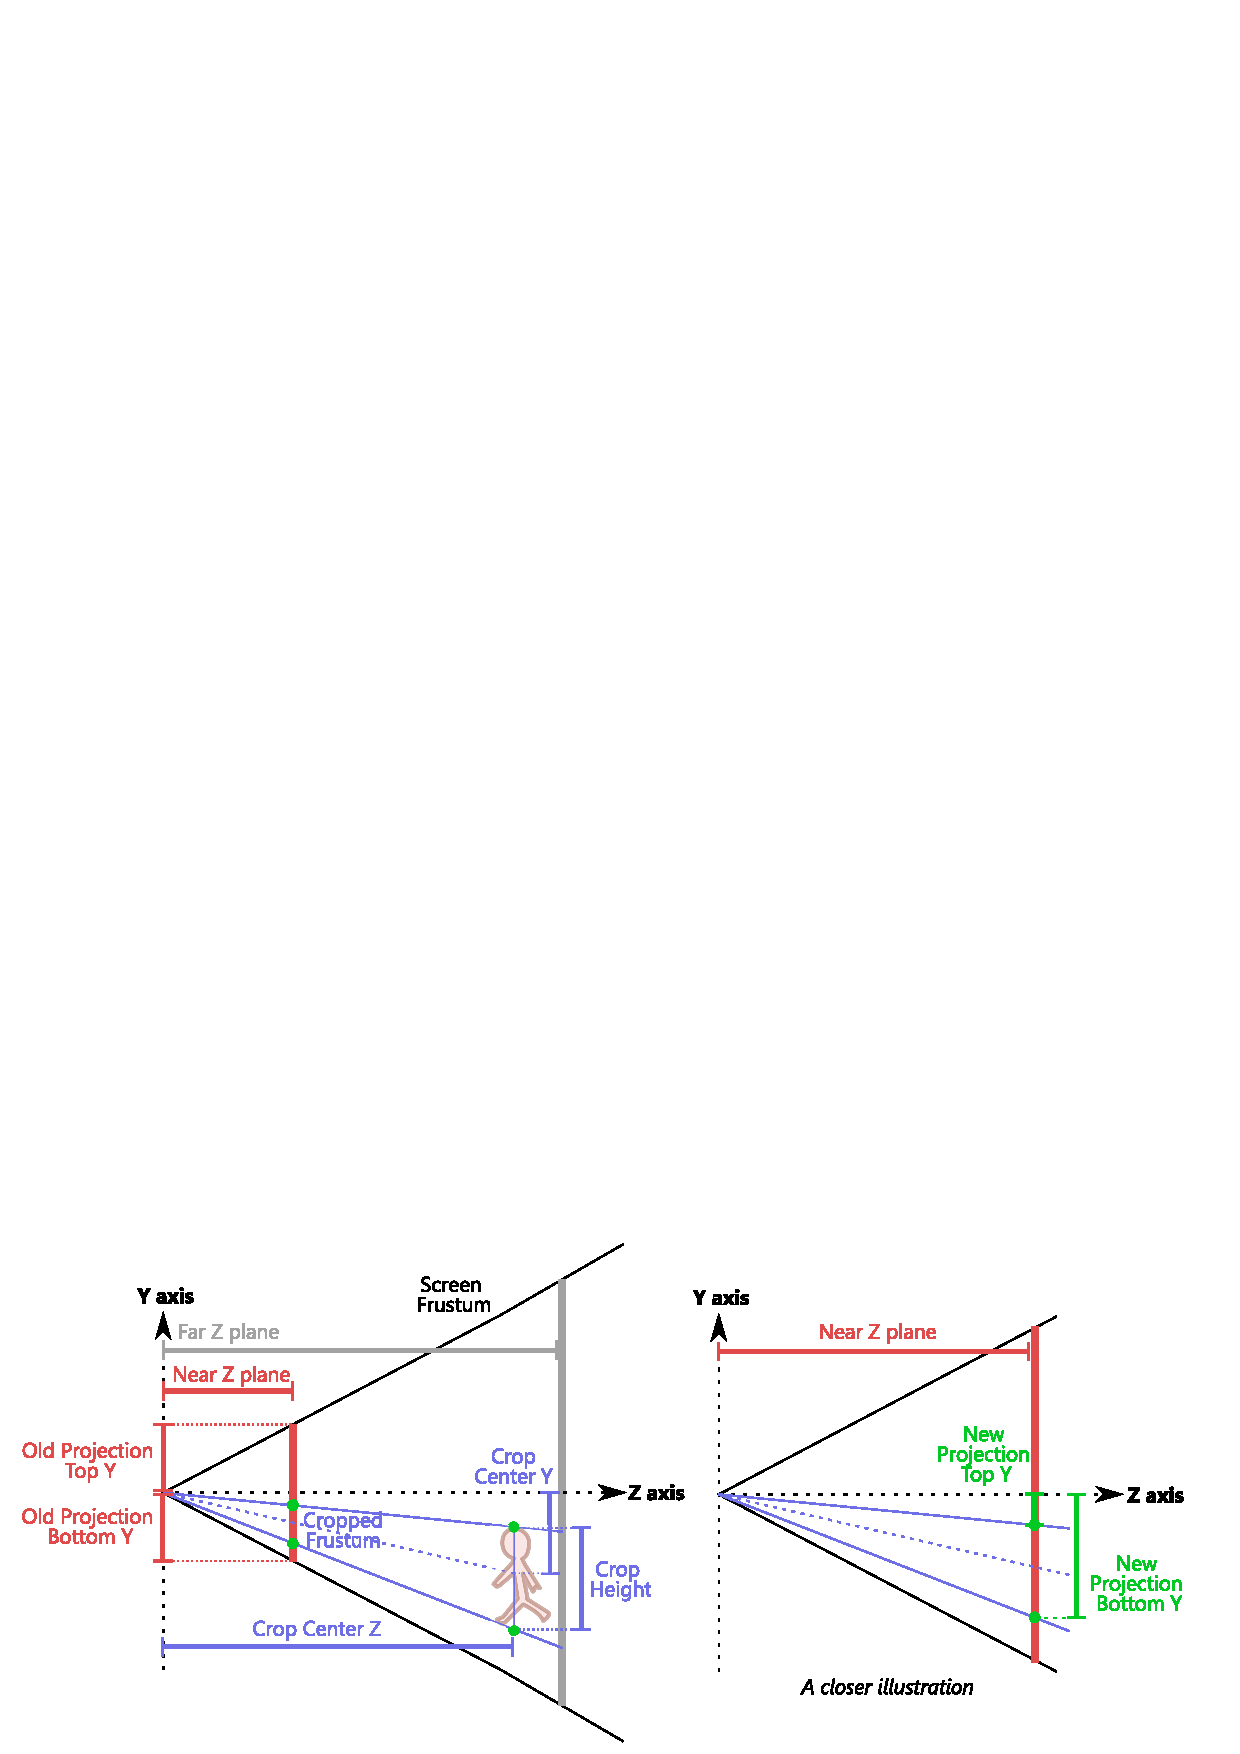
\includepdf[width=\textwidth]{\imgfp/dynamic_crop/dynamic_crop}
	\caption{A 3D space with origin at the camera, and axes aligned with camera directions ($x$ - right, $y$ - top, $z$ - front). The figure shows a slice of this space with $x=0$, illustrating the dynamic projection crop. \textit{(Left)} The near plane of the old screen frustum is defined by a $z$ distance (arbitrary), and $x$/$y$ coordinates of the frustum borders (top/bottom coordinates on illustration). \textit{(Right)} To make the projection cropped around the avatar body, we compute an axis-aligned bounding box of the body, then project its spans onto the near plane, obtaining top/bottom borders, defined by intersection coordinates of the projection lines and the old near plane. The new frustum will have the same near and far planes as the old one, to ensure preservation of perspective.}
	\label{fig:dynamic_crop_math}
\end{figure}

%TODO
\alert{TODO: Explain in details}
\begin{itemize}
	\item SMPL-X inference on mobile
	\begin{itemize}
		\item  "ON CPU" -- Pre-inference of shape blendshapes into a default posed mesh, load as a GPU buffer into OpenGL
		\item "ON CPU" -- Pre-compute indices of 12 the most influential joints for every mesh vertex, pre-load them on GPU as well.
		\item "ON CPU" -- On each frame compute posed joints (i.e. 55 rotation matrices): unwrap 3 axis angles into matrices following Rodrigues formula for rotations, multiply matrices in topological order to combine rotations of multiple joints. Load the matrices on GPU as shader uniforms (shared by all vertices)
		\item "ON GPU Vertex Shader" -- find a weighted sum of rotation matrices for each vertex (only 12 matrices to add up, using the most influential joints indices, without it 55 matrices would need to be added per each vertex). Project each vertex onto image, using a combination of extrinsic and intrinsic matrices of the camera.
	\end{itemize}
	\item Rasterization with a neural texture and quantization overcoming OpenGL limitations
	\begin{itemize}
		\item OpenGL can only render images with 4 channels RGBA. If rendering 16 channels naively, it requires to render 4 images with 4 channels, then send them to the DNN, and permute channels from 4xHxWx4 to 1xHxWx16, which is long to do on each frame (takes up to 20 ms)
		\item Using quantization, we can let network accept each channels as an 8-bit integer number. Then in OpenGL we can quantize in parallel rasterized pixels from 4-byte floats to 1-byte integers, pack them together with 4 neural channels per OpenGL channel, and then we do not need to permute channels, the input goes straight into the DNN and the first convolution starts immediately. The visual quality loss is not drastic
		\item Using quantized numbers, it also opens an opportunity to run on Digital Signal Processor (DSP), which is designed to do fast quantized computations (mainly because of bit-fiddling shortcuts possible with integers, and not with IEEE floating point numbers). Overall the performance is more than real-time with up to 640 px resolution
	\end{itemize}
	\item Dynamic camera frustum cropping
		\begin{itemize}
			\item Around view span -- On every frame compute coordinates of joints in camera space, find a XY-bounding box for them. Project bounds of this box onto the image, and find adjustments of top-bottom-left-right-near-far parameters of the camera frustum. Calculate a new projection matrix to fit only the bounding box of the avatar. Rasterize an input frame with this matrix. Infer the network and place the output using offset computed from the updated projection matrix
			\item Auto-zoom to reducing frame waste -- detect if bounding box of joints is cut off by the mobile screen. Zoom in the projection matrix to the avatar to compensate cut off parts. This will allow to see the avatar parts rendered in bigger resolution (thus DNN has to be trained on zoom scale too)
		\end{itemize}
	
	\item \alert{TODO: parallelization}
\end{itemize}

\section{Improving quality of synthesized images}\label{methods:zooms}
\begin{figure}
	\centering
	\begin{subfigure}[b]{0.48\textwidth}
		\centering
		\includegraphics[width=\textwidth]{\imgfp/cam_augs/img}%
		\caption{}
		\label{fig:cam_aug:before}
	\end{subfigure}
	\begin{subfigure}[b]{0.48\textwidth}
		\centering
		\includegraphics[width=\textwidth]{\imgfp/cam_augs/cam}%
		\caption{}
		\label{fig:cam_aug:after}
	\end{subfigure}
	\caption{(\protect\subref{fig:cam_aug:before}) Implementation of zooming using image-space augmentations. The body mesh is rasterized in full-body, the ground truth is transformed once to be in an alignment with the rasterization. Then both are magnified, loosing a lot of quality. (\protect\subref{fig:cam_aug:after}) Using camera-space augmentations, the virtual camera used for rasterization replicates zooming by moving towards the avatar. The input image can be made arbitrarily sharp. The ground truth image is still transformed with image-space augmentations, but only once, preserving a bit of quality. }
	\label{fig:cam_aug}
\end{figure}

\begin{figure}
	\centering
%	\begin{subfigure}[b]{0.3\textwidth}
%		\centering
		\includegraphics[width=\textwidth]{\imgfp/smplx/one-joint-vertices}%
%		\caption{}
%		\label{fig:smplx:4-joints-vertices}
%	\end{subfigure}
%	\begin{subfigure}[b]{0.69\textwidth}
%		\centering
%		\includegraphics[height=5cm]{\imgfp/smplx/vert2joint}%
%		\caption{}
%		\label{fig:smplx:all-joints-vertices}
%	\end{subfigure}
	\caption{Assignment of mesh vertices (red) to body joints (blue). For each vertex, we take the joint with the most significant skinning weight from SMPL-X body model, that determines how movement of the joint affects the given vertex's movement. We use this assignment to select mesh vertices as centers of camera-space augmentations. We speculate that choosing vertices rather than plain joints improves augmentations variance and decreases overfitting.}
	\label{fig:smplx-vert2joint}
\end{figure}

The baseline DNN architecture \cite{dnn:stylepeople21} proved to be sufficient to render FB images of avatars. However, we found out that the rendering network cannot reliably render parts on the body that were never seen during training, most commonly under boots surface, and top of the head. At best, these places can be rendered as random patches of color, e.g. from clothes or skin. Intuitively it is so, because in these areas the neural texture will contain default values during the whole training process. If the renderer learns quickly enough to map such default values to skin or clothes, the chance is that the texture overall will not move much away from the defaults. Although the unseen parts are not rendered correctly from reconstruction point of view, it does not hurt overall accuracy. On the other hand, there is a chance that the neural texture will significantly move away from the default initialization. Thus, after many epochs the default values contained in the unseen parts will be outliers that the renderer does not expect to see. This may trigger it to render abnormal color or fail segmentation prediction. Attempts on dealing with this artifact will be given shortly after.

Besides the unseen parts, after launching the model
\alert{TODO: Motivation and pre-conclusions}

Researched adjustments:
\begin{itemize}
	\item Camera space affine augmentations module (for Python) to eliminate need of augmenting prerasterized frame (which will lead to quality loss on strong zooms)
	\item Zooming to different joints (or mesh vertices) with different scale range 
	\item Regularization of Batch Normalization layers to prevent overfit (and Spurious Correlations as result): collecting statistics on FB scale only, or on zoom scale only; using current statistics to train or not
	\item Accumulating gradients for more than 1 batch before making optimization step
	\item Adam Optimizer without 1st momentum in neural renderer, discriminator
	\item Fine tuning a zoom-trained model on FB to restore FB quality and to preserve neural texture high frequency details
	\item Other normalization layers: Instance norms, Group norms, No norms
	\item Adam optimizer of the neural texture - do not decay momentum of pixels with 0 analytic gradient (unseen in the current batch)
	\item Capacity of neural texture, encoder, decoder
	\item Gradient norm clipping
	\item Learning rate scheduling with warmup and later annealing
	\item Concatenate input neural image to deeper activations of the encoder
	\item More strong affine augmentations 
	\item Batch normalization without learned affine parameters, or without tracking running statistics 
	\item Single-scale neural texture, compared to multiscale-texture
	\item Homogeneous augmentations in a single optimization batch (to prevent mixing of statistics)
	\item Disabling GAN losses
	\item Initializing neural texture training from a stable pretrained checkpoint, or random noize, compared to spectral initialization
	\item Disable discriminator on zooms, or disable discriminator on FB
	\item Equal loss weights
	\item Using scale probability distribution to prioritize FB scale and show close-up and far-out ever so rarely
	\item Dropout2d to nullify random feature maps after convolutions: in encoder, in decoder, in both
	\item Change input rasterization background to not 0 (which is a valid value on the neural texture), but to ntex.abs()*2
	\item Add gaussian noize to input rasterization, or neural texture, or ground truth
	
\end{itemize}

%\begin{figure}[!htbp]
%	\centering
%	\begin{lstlisting}[
	%		language=C++,
	%		numbers=none,
	%		basicstyle=\ttfamily,
	%		keywordstyle=\color{NavyBlue}\textbf,
	%		frame=single,
	%		extendedchars=true,
	%		tabsize=4,
	%		morekeywords={interface, string},
	%		]
	%public interface IVisualizer
	%{
		%	string GetDescription();
		%	void VisualizeModel(Stream model, ModelMetaBase modelMeta, 
		%	Stream materialLibrary, Stream[] materialFiles);
		%	void Shutdown();
		%} 
	%	\end{lstlisting}
%	%	\captionsetup{justification=centering}
%	\caption{Blah blah example}\label{res:code:example}
%\end{figure}